% Created 2024-07-12 Fri 17:34
% Intended LaTeX compiler: pdflatex
\documentclass[presentation]{beamer}
\usepackage[utf8]{inputenc}
\usepackage[T1]{fontenc}
\usepackage{graphicx}
\usepackage{longtable}
\usepackage{wrapfig}
\usepackage{rotating}
\usepackage[normalem]{ulem}
\usepackage{amsmath}
\usepackage{amssymb}
\usepackage{capt-of}
\usepackage{hyperref}
\institute[UniPD]{Master degree in Computer Science \mbox{}\\ \mbox{}\\ Università degli studi di Padova}
\usepackage{preamble}
\usepackage{commands}
\usetheme{CambridgeUS}
\author{Luca Zaninotto}
\date{03 Jul 2024}
\title[Decidability in abstract semantics]{Some decidability questions in abstract program semantics}
\hypersetup{
 pdfauthor={Luca Zaninotto},
 pdftitle={Some decidability questions in abstract program semantics},
 pdfkeywords={Abstract interpretation, Program semantics},
 pdfsubject={},
 pdfcreator={Emacs 29.4 (Org mode 9.6.15)}, 
 pdflang={English}}
\usepackage{biblatex}
\addbibresource{/home/luser/uni/tesi/presentazione/references.bib}
\begin{document}

\maketitle

\section{Introduction}
\label{sec:org3c03407}
\begin{frame}[label={sec:orgfb48c15}]{The cost of software failures}
\begin{columns}
\begin{column}{0.45\columnwidth}
\begin{figure}[htbp]
\centering
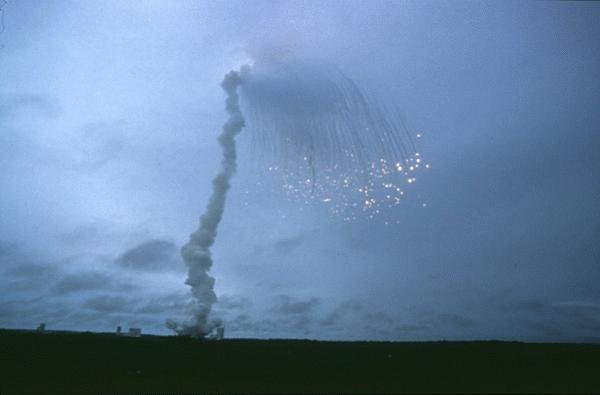
\includegraphics[width=\textwidth]{./images/ariane5.jpg}
\caption{Ariane 5 crash, circa 370mln\$ in damages}
\end{figure}
\end{column}
\begin{column}{0.45\columnwidth}
\begin{itemize}
\item Testing and careful design might not be enough.
\item Formal methods can help, by providing strong guarantees. \pause
\item We focus in particular on \alert{Abstract interpretation}.
\end{itemize}
\end{column}
\end{columns}
\end{frame}
\begin{frame}[label={sec:orgf8959c9}]{Abstract interpretation}
Given a program semantics, abstracts its behaviour and provide an
over-approximation of the program semantics
\begin{figure}
  \centering
  \begin{tikzpicture}
    \node (concrete) at (-1.2,1) {\(\mathcal{C}\)};
    \draw (0,0) ellipse [x radius=1cm, y radius=2cm];

    \pause
    \node (abstract) at (6.2,1) {\(\mathcal{A}\)};
    \draw (5,0) ellipse [x radius=1cm, y radius=2cm];

    \pause
    \node [red] (concel) at (0,1) {\textbullet};
    \node [blue] (abstel) at (5,1) {\textbullet};
    \draw (concel) edge[->,bend left=10] node[above]{\(\abstr\)} (abstel);

    \pause
    \node [codegreen] (abstres) at (5,-1) {\textbullet};
    \node (txt) at (7,0) {\rmfamily\tiny Abstract};
    \node (txt1) at (7,-.3) {\rmfamily\tiny computation};
    \draw [codegreen, ->] (abstel) edge[dashed, bend left=10] (abstres);

    \pause
    \draw [codegreen, thick] (0,-1) ellipse [x radius=.3cm, y radius=.5cm];
    \fill [codegreen, very nearly transparent] (0,-1) ellipse [x radius=.3cm, y radius=.5cm];
    \draw [codegreen] (abstres) edge[bend left=5] (0,-0.5);
    \draw [codegreen] (abstres) edge[bend left=10] (0,-1.5);
    \node (gamma) at (2,-1.25) {\(\concr\)};

    \pause
    \node (concres) at (0,-1.3) {\textbullet};
    \draw [->] (concel) edge[dashed, bend right=10] (concres);
    \node (txt2) at (-2,0) {\rmfamily\tiny Concrete};
    \node (txt3) at (-2,-.3) {\rmfamily\tiny computation};

    \node [blue] (txt4) at (-2, -1.3) {\scriptsize Soundness};

    \pause
    \node (txt5) at (7,-2) {\tiny Does it terminate?};
    \draw [->] (txt5) edge[bend right=10] (txt1);
    \onslide<1->
  \end{tikzpicture}
\end{figure}
\end{frame}
\begin{frame}[label={sec:org22b6be5},fragile]{Analyzer termination is not guaranteed}
 Consider the C-like program
\begin{lstlisting}[language=C,label= ,caption= ,captionpos=b,numbers=none]
int x = 0;
while(true) {
  x++;
}
\end{lstlisting}
A concrete semantics that collects variables values diverges
\begin{center}
  \([\var\mapsto 0]\) \pause
  \(\to \{[\var\mapsto 0], [\var\mapsto 1]\}\) \pause
  \(\to^* \{[\var\mapsto n] \mid 0 \leq n \leq k, k\in\n\}\) \pause
   \(\to\dots\)
 \end{center}
Intervals would also diverge
\begin{center}
  \([\var\mapsto [0,0]]\) \pause
  \(\to [\var\mapsto [0,1]]\) \pause
  \(\to^* [\var\mapsto [0,k]]\) with \(k\in\n\) \pause
   \(\to\dots\)
 \end{center}
\end{frame}
\begin{frame}[label={sec:org269b413}]{Goal}
\begin{itemize}
\item Establish if some abstract semantics are computable.
\item Focus on non-relational domains:
\begin{enumerate}
\item \alert{Interval domain} \(\inte \defin (\Var \mapsto \Int)\):
\(\var\mapsto\)range where \(\var\) can vary \onslide<2>
\alert{Computable}
\item \onslide<1-> \alert{Non-relational collecting domain} \(\bCnr \defin
        (\Var \mapsto \poset{\z})\): \(\var\mapsto\) set of possible
values of \(\var\). \onslide<2> \alert{Partial results}
\end{enumerate}
\end{itemize}
\end{frame}
\section{Outline}
\label{sec:org9bb4d0e}
\begin{frame}[label={sec:orgf854a45}]{Outline}
\begin{enumerate}
\item \(\imp\) language and its semantics
\item Non relational abstract domains
\item Computing the abstract semantics
\item Results and future work
\end{enumerate}
\end{frame}
\section{Imp}
\label{sec:org3f322a0}
\begin{frame}[label={sec:orgfbc9ae4}]{Grammar}
\begin{itemize}
\item Minimal core of an imperative language;
\item Turing complete;
\item Based on Kleene algebras with tests.
\end{itemize}


\begin{align*}
  \expr \ni \com[e] ::= & \; \var \in I \mid \var := k \mid \var := \var[y] + k \\
  \imp \ni \com[C] ::= & \; \com[e] \mid \com + \com \mid \com ; \com \mid \com^* \mid \fix{\com}
\end{align*}

\begin{itemize}
\item while \(b\) do \(\com\) \(\implies \fix{b \seq \com} \seq
     \neg b\)
\item if \(b\) then \(\com_1\) else \(\com_2\) \(\implies (b \seq
     \com_1) \ndet (\neg b \seq\com_2)\)
\end{itemize}
\end{frame}

\begin{frame}[label={sec:orgffbc4ff}]{Concrete semantics}
\begin{align*}
  \sem{\com[e]} X & \defin \{\bsem{\com[e]} \rho \mid \rho \in X,
  \bsem{\com[e]} \rho \neq \bot\} \\
  \sem{\com[C_1] + \com[C_2]} X & \defin \sem{\com[C_1]} X \cup \sem{\com[C_2]} X \\
  \sem{\com[C_1] ; \com[C_2]} X & \defin \sem{\com[C_2]}(\sem{\com[C_1]} X) \\
  \sem{\com[C^*]} X & \defin \bigcup_{i \in \n} \sem{\com[C]}^i X \\
  \sem{\fix{C}} X & \defin \lfp(\lambda Y \in\poset{\env} . (X \cup \sem{\com}Y))
\end{align*}
\begin{itemize}
\item Collecting semantics.
\item Finiteness and termination are undecidable because of Rice.
\end{itemize}
\end{frame}

\begin{frame}[label={sec:orgad4f958}]{Undecidability of collecting semantics}
Given an initial state \(\rho \in \poset{\env}\) and a program
\(\com\)
\begin{itemize}
\item Does the computation of \(\sem{\com}\rho\) terminate?
\item Is \(\sem{\com}\rho\) finite?
\end{itemize}

\pause
Both \alert{undecidable} because of Rice's Theorem.
\end{frame}
\section{Non-relational domains}
\label{sec:orgf95f6b7}
\begin{frame}[label={sec:orga06e8d3}]{Interval domain}
\begin{equation*}
  \Int \defin \{[a,b] \mid a \in \z \cup \{-\infty\}, b\in\z\cup\{+\infty\} \land a \leq b\}
\end{equation*}
\begin{itemize}
\item Variables map to an interval \([\var \mapsto [-1,1], \var[y]
     \mapsto [0,0], \dots]\)
\item \alert{Non-relational}: relations beween variables (e.g., \(\var =
     3*\var[y]\)) are not modelled
\item Computation of fixpoints non trivial
\end{itemize}
\end{frame}
\begin{frame}[label={sec:org2065ba8},fragile]{Infinite chains}
 \begin{lstlisting}[language=imp,label= ,caption= ,captionpos=b,numbers=none]
x := 0; fix(true; x++)
\end{lstlisting}
\begin{itemize}
\item Computation does not halt
\begin{equation*}
  [\var\mapsto 0] \to \{[\var\mapsto 0], [\var\mapsto 1]\} \to \dots \to \{[\var\mapsto n] \mid n\in\n\}
\end{equation*}
\item Analysis does not halt either
\begin{equation*}
  [\var\mapsto[0,0]] \to [\var\mapsto[0,1]] \to \dots \to [\var\mapsto[0,\infty]]
\end{equation*}
\item Problem: iterating over an infinite chain in the domain
\begin{equation*}
  [0,0] \sqsubseteq [0,1] \sqsubseteq \dots \sqsubseteq [0,\infty]
\end{equation*}
\end{itemize}
\end{frame}
\begin{frame}[label={sec:org818476e},fragile]{Widening and narrowing}
 \begin{itemize}
\item Common approach: widening \(\widen\)
\item Widening over-approximates a result. Example
\begin{lstlisting}[language=imp,label= ,caption= ,captionpos=b,numbers=none]
x := 0; fix(x < 10; x++);
\end{lstlisting}
\begin{itemize}
\item \alert{Precise analysis} (not guaranteed to halt): \([\var\mapsto[0,10]]\)
\item \alert{Analysis with widening} (halts): \([\var\mapsto[0,\infty]]\))
\end{itemize}
\end{itemize}
\end{frame}
\begin{frame}[label={sec:org6a31266}]{The problem}
\begin{problem}
Can we compute the precise interval semantics while ensuring the
termination of the analyzer?
\end{problem}
\end{frame}
\begin{frame}[label={sec:org19ffb0a}]{Bounding the interval domain}
Consider the behavior of some variable \(\var\) while computing
\begin{equation*}
  \semi{\fix\com}\eta = \lfp(\lambda\mu . (\eta\sqcup\semi{\com}\mu))
\end{equation*}
\begin{figure}
  \centering
  \begin{tikzpicture}
    %% Axes
    \draw[help lines, <->] (-5,0) -- (5,0);
    \draw[help lines] (0,-.5) -- (0,.5);
    \draw[help lines] (-4,.1) grid (4,-.1);
    \node (x) at (-5,1) {\footnotesize\(\var\)};

    %% x initial state
    \onslide<1>{\node [blue] (a) at (-.81,0) {$[a_1$};}
    \onslide<1>{\node [blue] (b) at (.3,0) {$b_1]$};}

    %% after some rounds
    \pause
    \node [blue] (a2) at (-1.81,0) {$[a_2$};
    \onslide<2>{\draw (a.north) edge[->, bend right=10] (-2,.3);}
    \onslide<2>{\node [blue] (b) at (.3,0) {$b_1]$};}

    \pause
    \onslide<3>{\draw (b.north) edge[->, bend left=10] (1,.3);}
    \onslide<3>{\node [blue] (b2) at (.81,0) {$b_2]$};}

    \pause
    \node [red,label={[font=\scriptsize,color=red]above:\(\low\)}]
    (low) at (-3,0) {[};
    \node [red,label={[font={\rmfamily\scriptsize},color=red]above:\(\upp\)}]
    (low) at (3,0) {]};
    \onslide<4>{\node [blue] (b3) at (.81,0) {$b_2]$};}

    \pause
    \onslide<5>{\draw (b2.south) edge[->,dashed,blue,bend right=10] (4,-.3);}
    \onslide<5>{\node [blue] (b4) at (3.81,0) {$b_3]$};}

    \pause
    \node [blue, thick] (b5) at (6,0) {$\infty]$};
    \draw [blue] (b4.south) edge[->] (b5.south);
    \onslide<1->
  \end{tikzpicture}
\end{figure}
\pause
\begin{itemize}
\item Bounds are determined by the program \(\com\) and the initial
environment
\item If a variable exceeds a bound the corresponding side of the
interval is pushed to infinity
\end{itemize}
\end{frame}
\begin{frame}[label={sec:orgd092f92}]{Bounding the interval domain}
By choosing \(\low,\upp\) appropriately
\begin{align*}
  \binte{\low}{\upp} \defin & \; \{[a,b] \mid a,b\in\z \land \low \leq a \leq b \leq \upp\} \\
  & \; \cup \{[a,+\infty] \mid a \geq \low\} \\
  & \; \cup \{[-\infty,b] \mid b \leq \upp\}
\end{align*}
it holds that
\begin{equation*}
  \semi{\com}\eta = \bsemi{\low}{\upp}{\com}\eta
\end{equation*}

Since \(\binte{\low}{\upp}\) does not contain infinite chains, the
termination trivializes.
\end{frame}
\begin{frame}[label={sec:orgaa0cd87}]{Non-relational collecting domain}
\begin{equation*}
  \bCnr \defin (\Var \to \poset{\z}) \cup \{\bot\}
\end{equation*}
\begin{itemize}
\item Variables mapped to a generic subset of integers.
\item Variable images are no longer convex.
\item We could only prove some partial results.
\end{itemize}
\end{frame}
\begin{frame}[label={sec:org7201876}]{Bounding the non-relational collecting domain}
\begin{equation*}
      \bposet{\low}{\upp}{\z} \defin \{S \subseteq \z \mid S \neq \emptyset \land \forall x \in S \quad \low \leq x \leq \upp\}
\end{equation*}
\begin{equation*}
  \btbCnr{\low}{\upp} \defin (\Var \to \bposet{\low}{\upp}{\z}) \cup \{\bot, \top\}
\end{equation*}
\begin{itemize}
\item Variables mapped to bounded subsets of \(\z\).
\item If some variable exceeds the bound than the whole analysis
results in the smashed \(\top\) element.
\item We can decide analysis termination. If the analysis halts then we
can provide the most precise abstract invariant (not in general).
\end{itemize}
\end{frame}
\section{Conclusions}
\label{sec:orgddde969}
\begin{frame}[label={sec:org4be2c18}]{Results}
\begin{itemize}
\item Interval analysis can be computed precisely in finite time
\begin{equation*}
  \semi[\inte]{\com}\eta = \semi[\binte{\low}{\upp}]{\com}\eta
\end{equation*}
\item For non-relational collecting semantics we can decide termination
of the analyzer.
\end{itemize}
\end{frame}
\begin{frame}[label={sec:orgbab2632}]{Future work}
\begin{itemize}
\item Generalize to more expressive languages (e.g. include non-linear
expressions).
\item Investigate the computability of non-relational collecting
semantics.
\item Generalize to other abstract semantics
\begin{itemize}
\item Non-relational
\item With a controlled amount of relationality
\end{itemize}
\end{itemize}
\end{frame}
\end{document}
